\section{Case study 3: real house} TBD

\subsection{Description of the house} TBD

\subsection{EnergyPlus model} TBD

\subsection{Simulation Results} TBD

\begin{figure}[h]
	\subfigure[Comparison of temperature of room $3$ obtained with DPC and ON/OFF controller.]{
		\label{F:Temperatures_small}
		\centering
		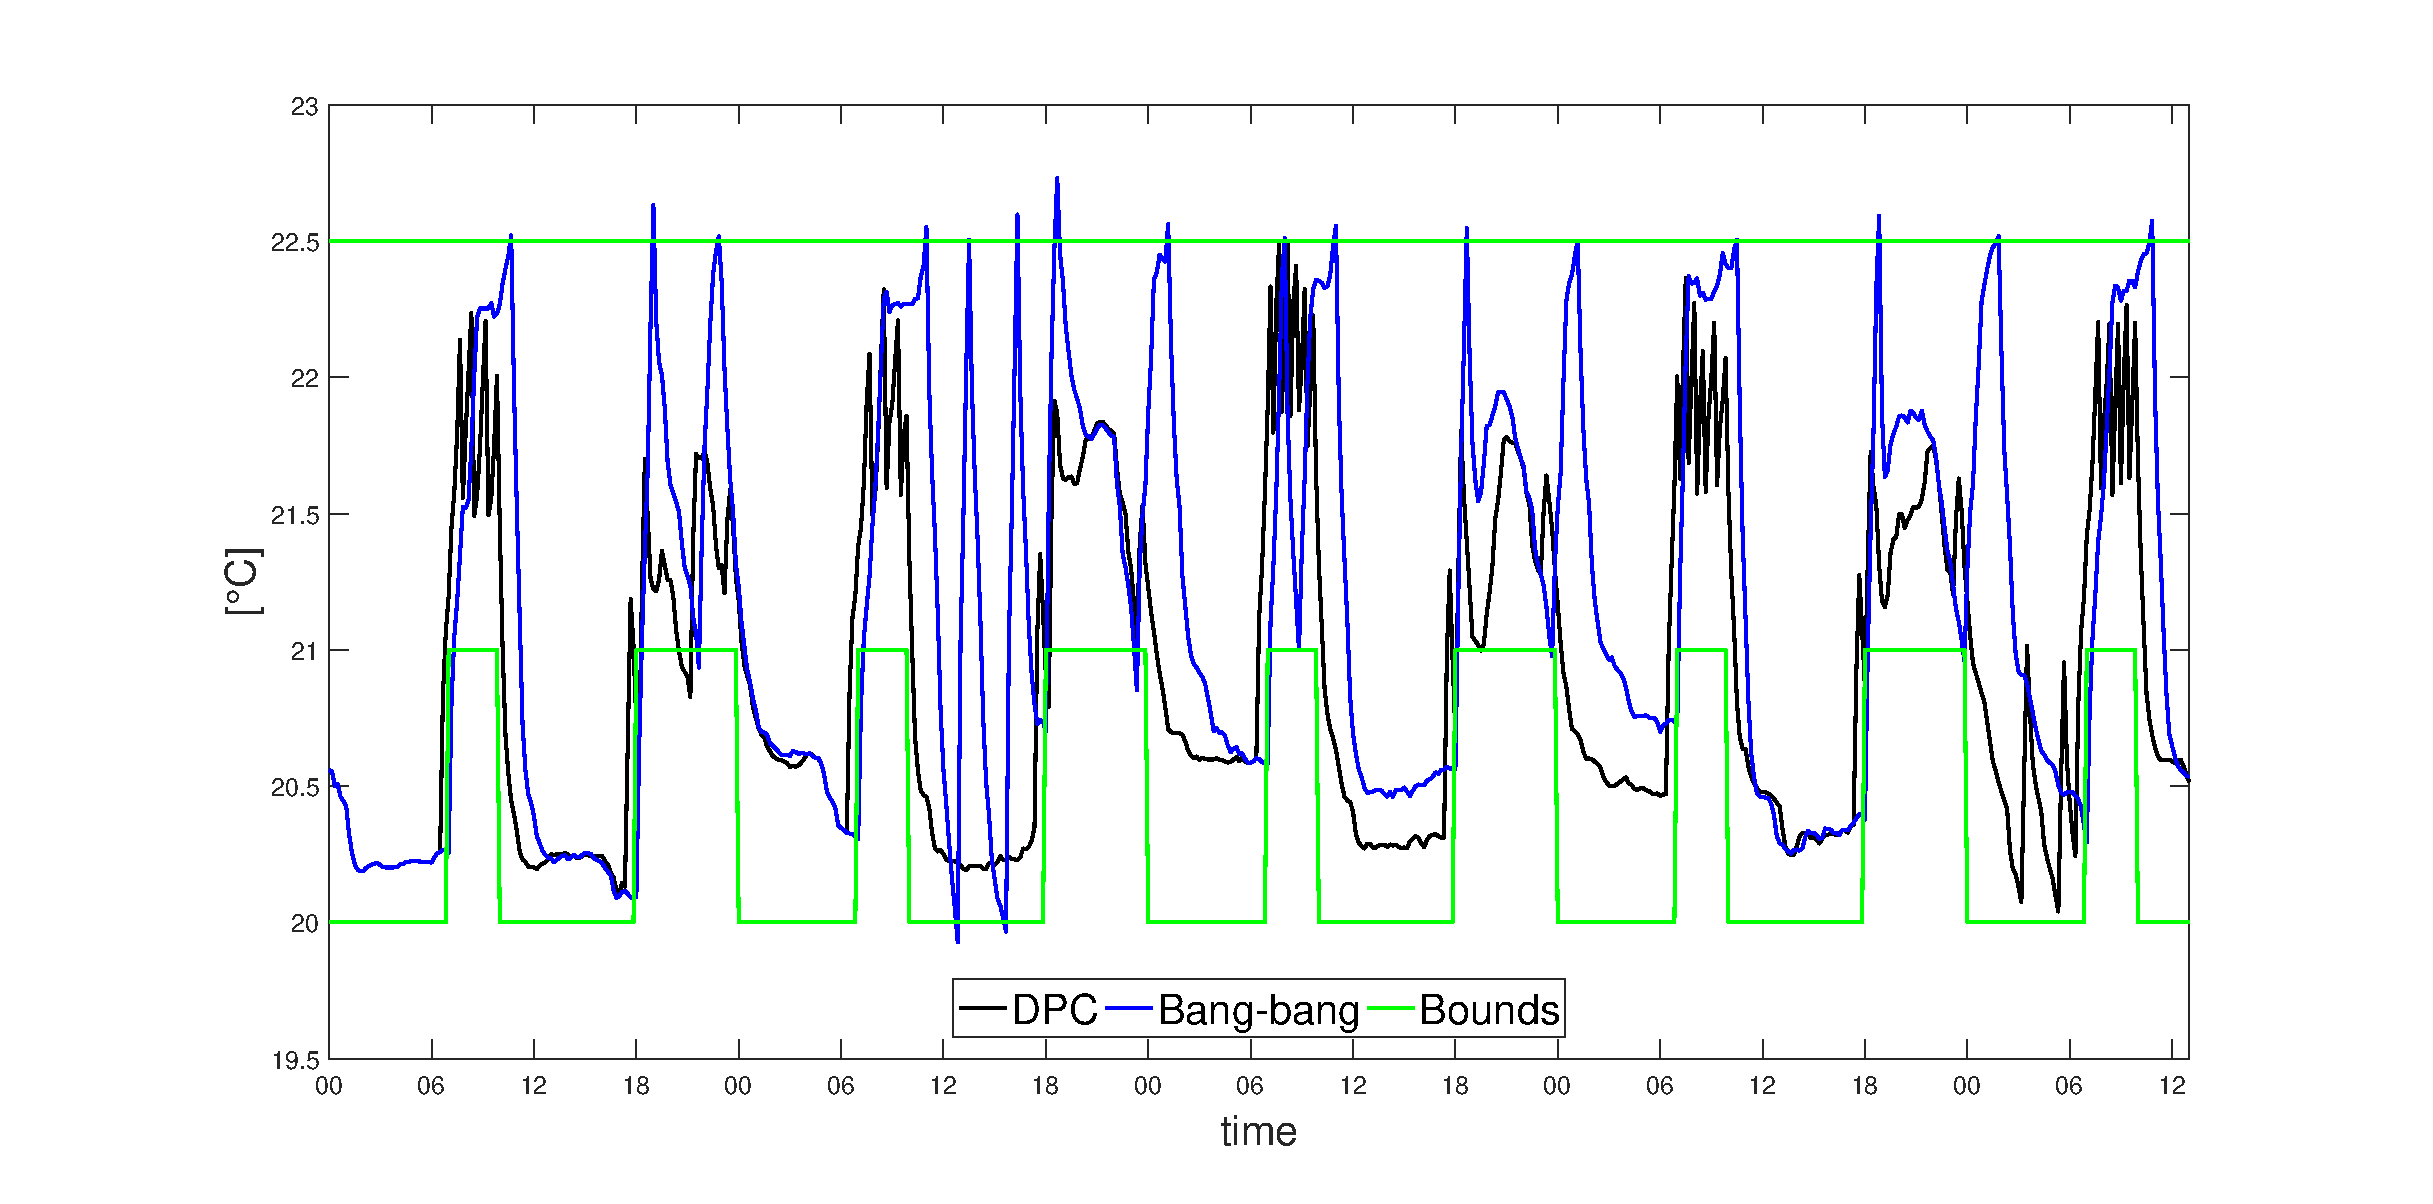
\includegraphics[width=22pc]{figures/Temperatures_small.eps}
	}
	\subfigure[Input schedules obtained from DPC and ON/OFF controller.]{
		\label{F:Inputs_small}
		\centering
		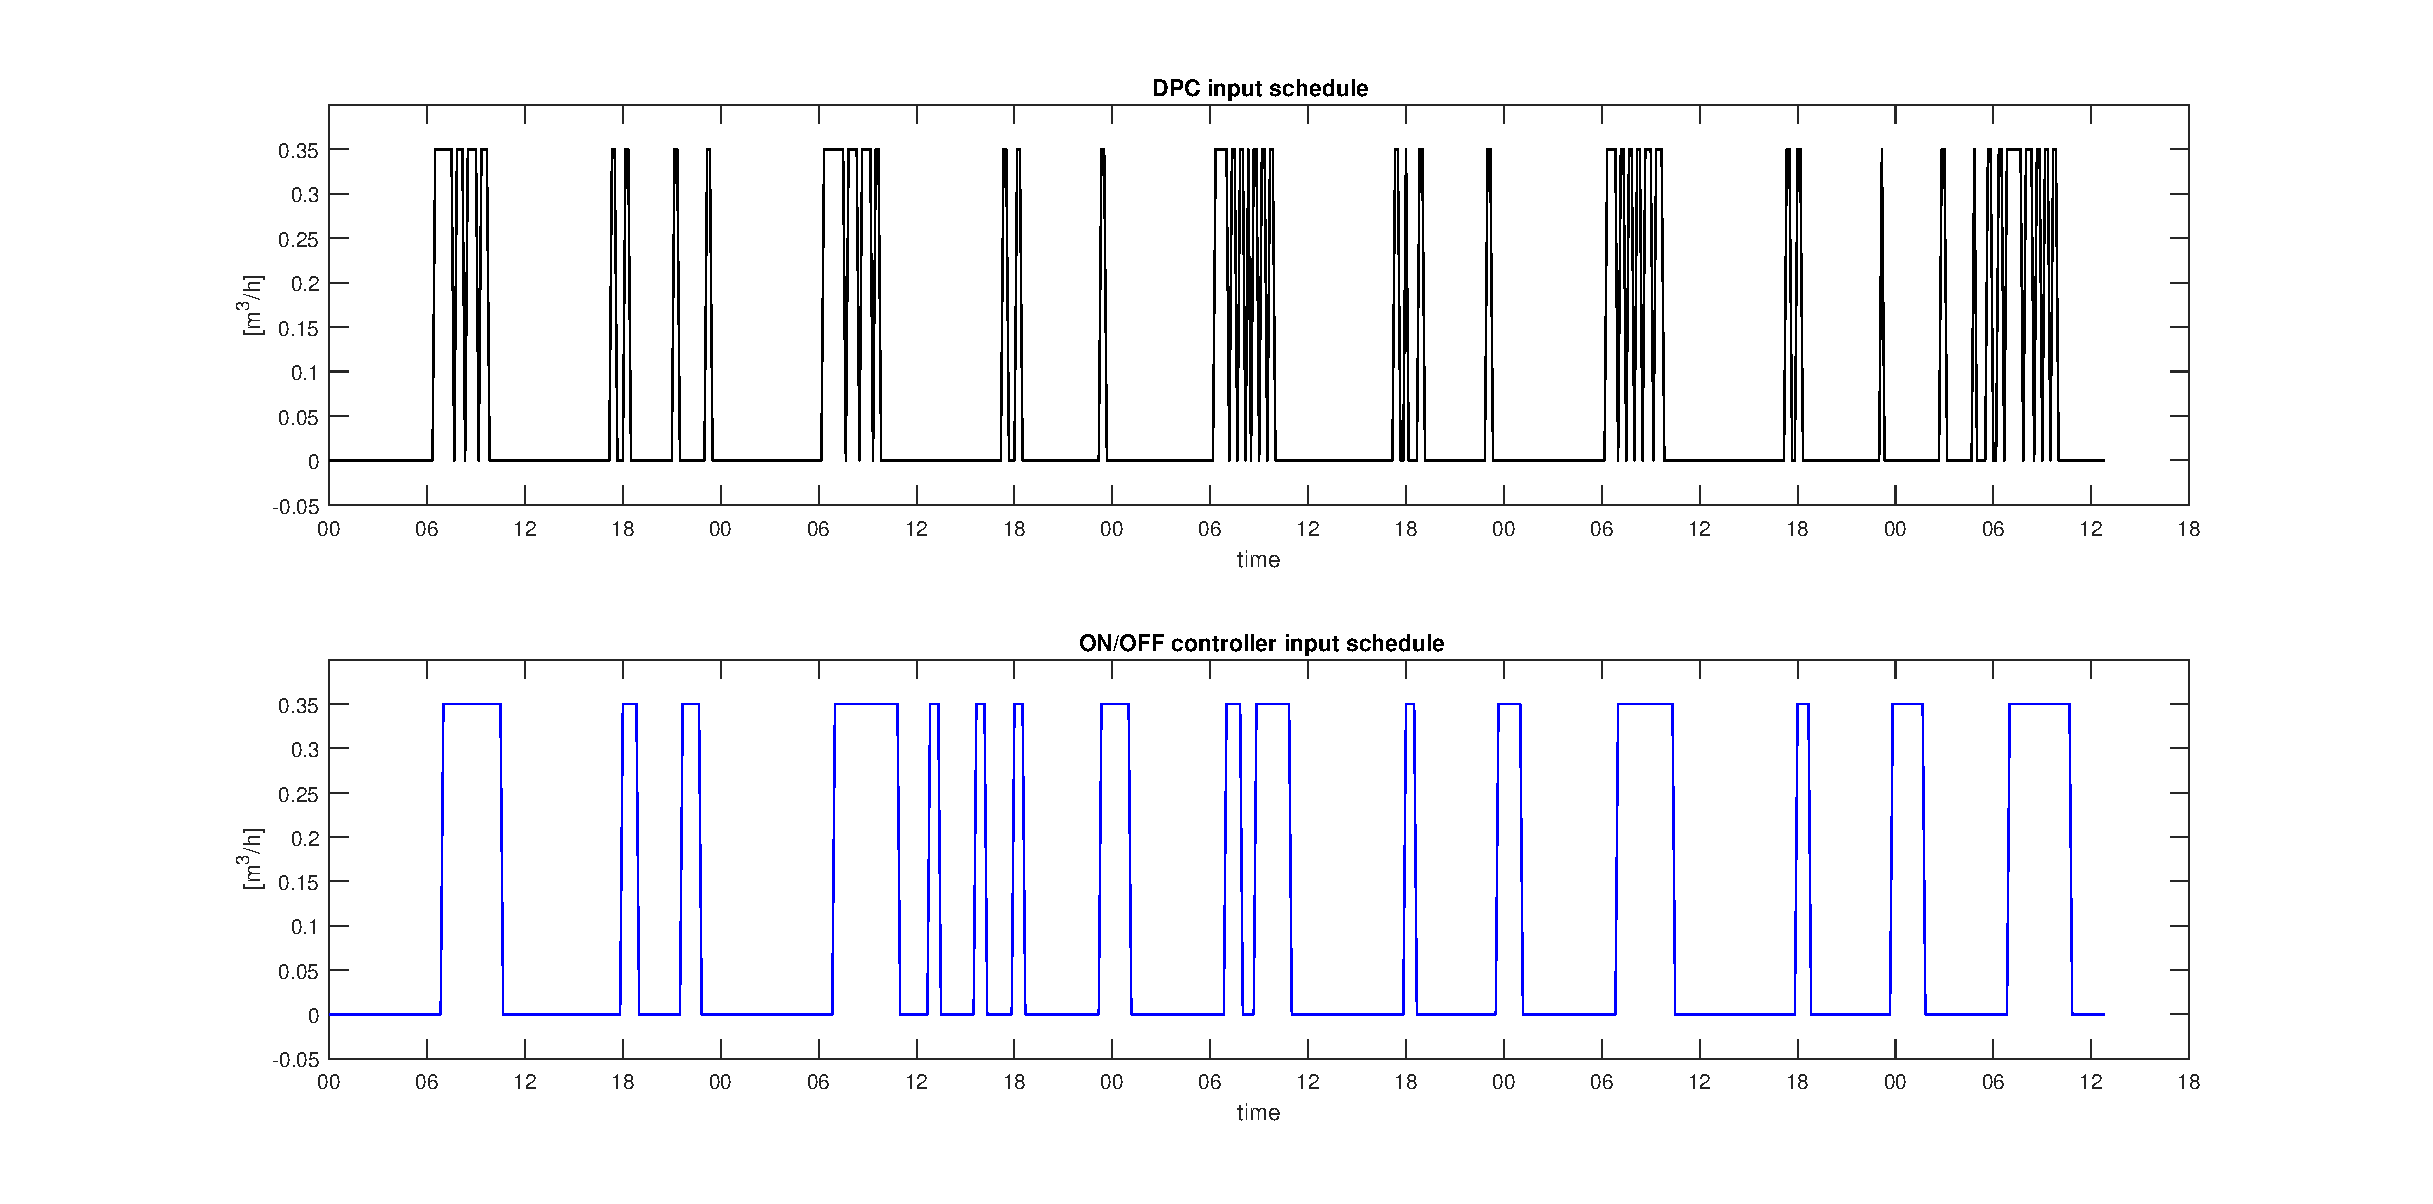
\includegraphics[width=22pc]{figures/Inputs_small.eps}
	}
	\subfigure[Energy consumption over the simulation period obtained with DPC and ON/OFF controller.]{
		\label{F:Energy_small}
		\centering
		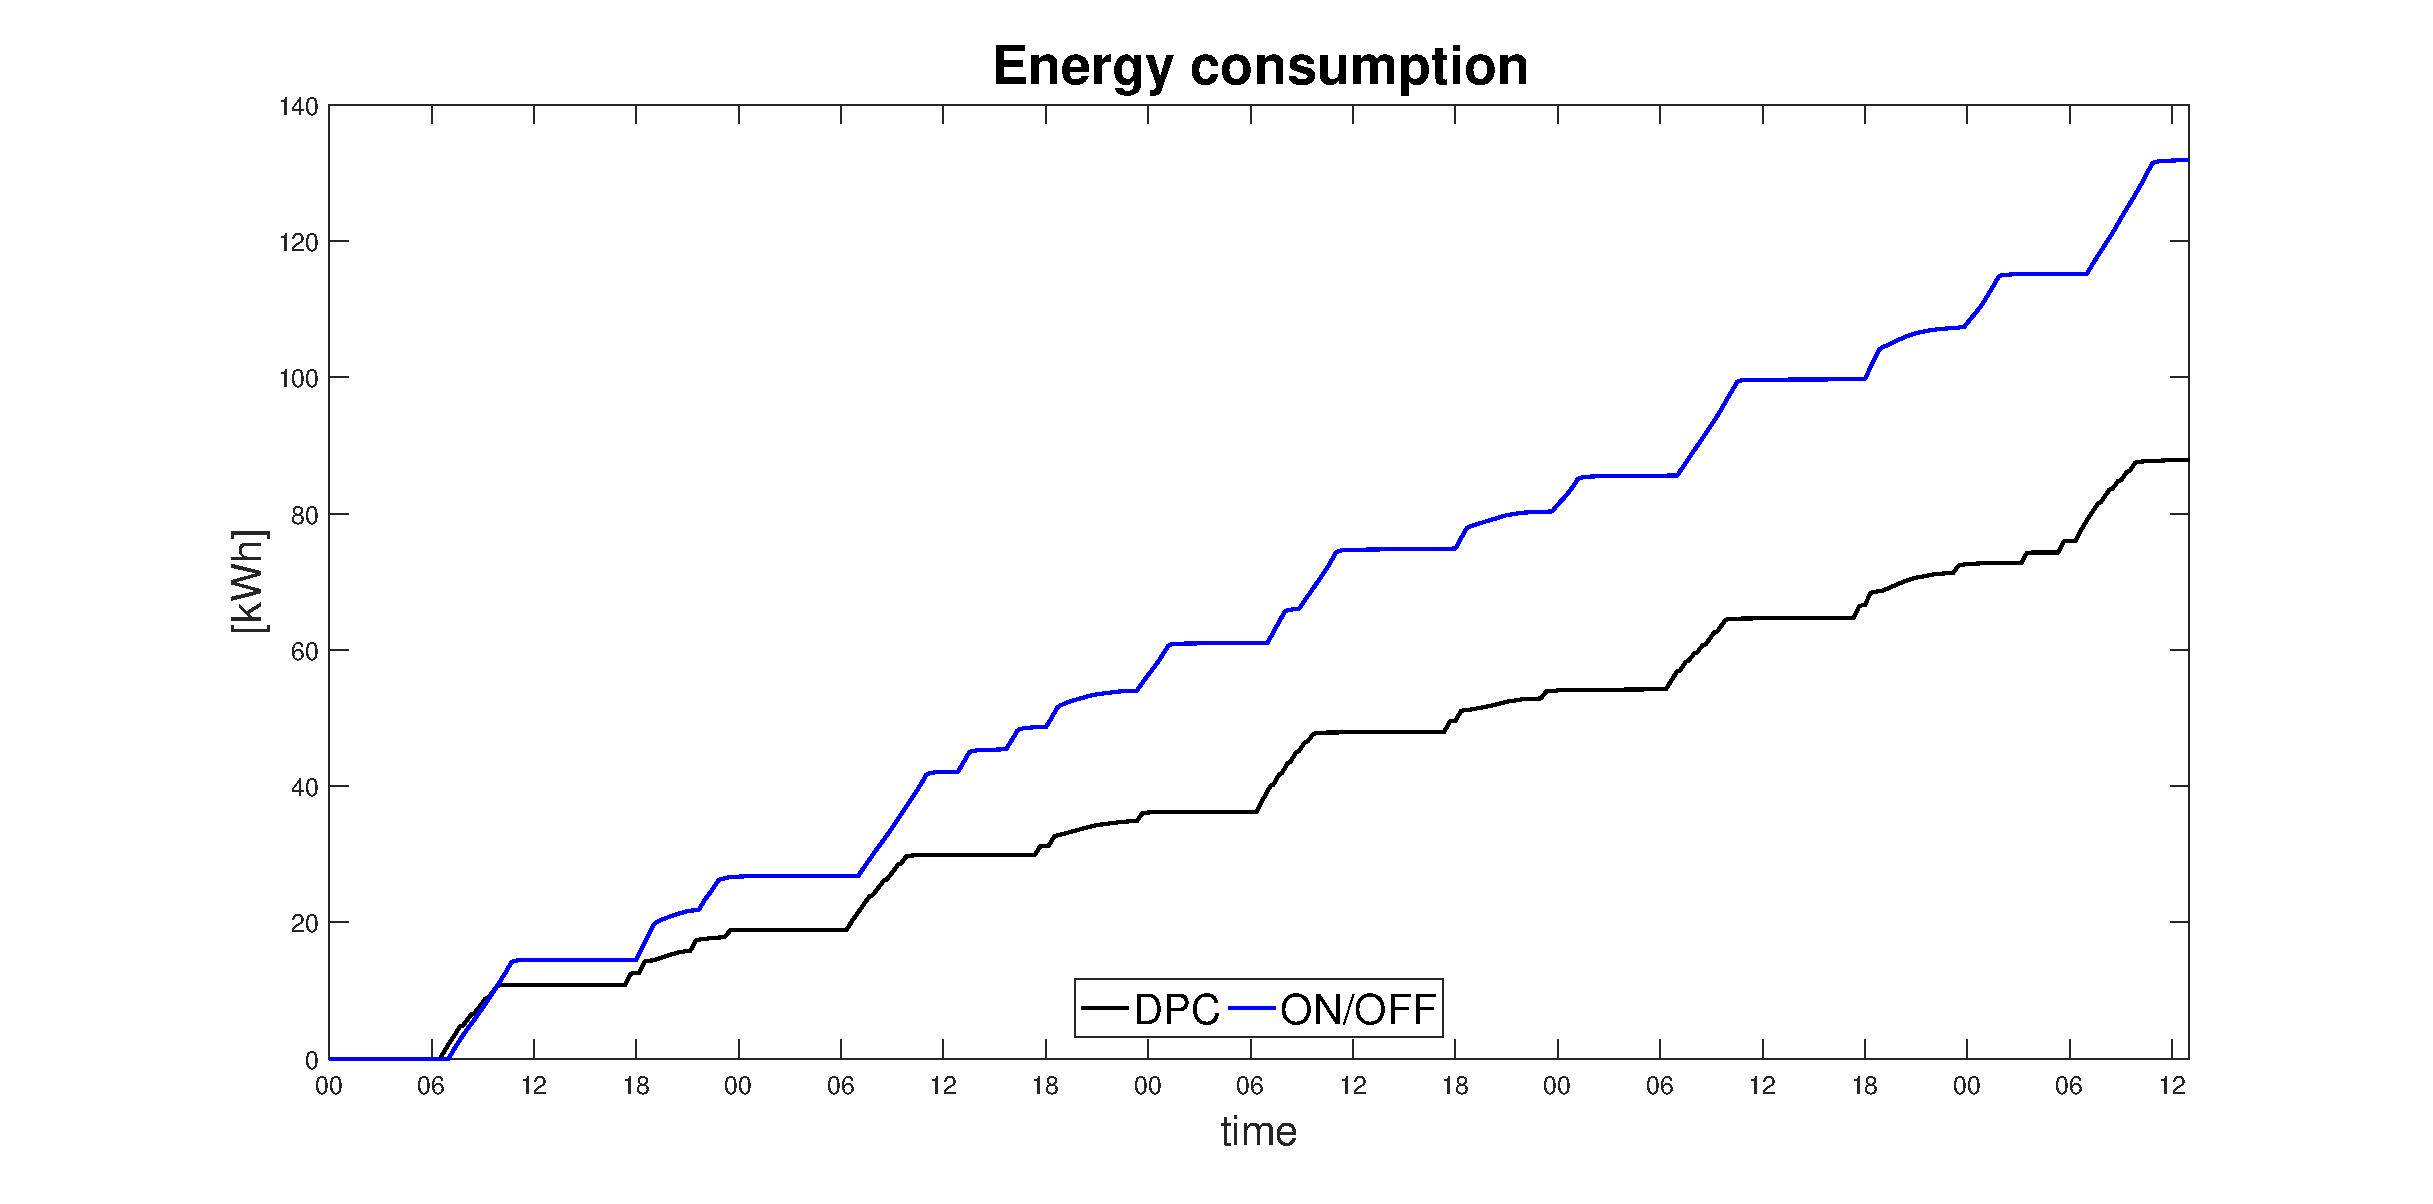
\includegraphics[width=22pc]{figures/Energy_small.eps}
	}
	\caption{Comparison of DPC and ON/OFF control performance.}
	\captionsetup{justification=centering}
	\label{F:Comparison_small}
\end{figure}

\begin{figure}[h]
	\subfigure[Comparison of temperature of room $3$ obtained with DPC and ON/OFF controller.]{
		\label{F:Temperatures_all}
		\centering
		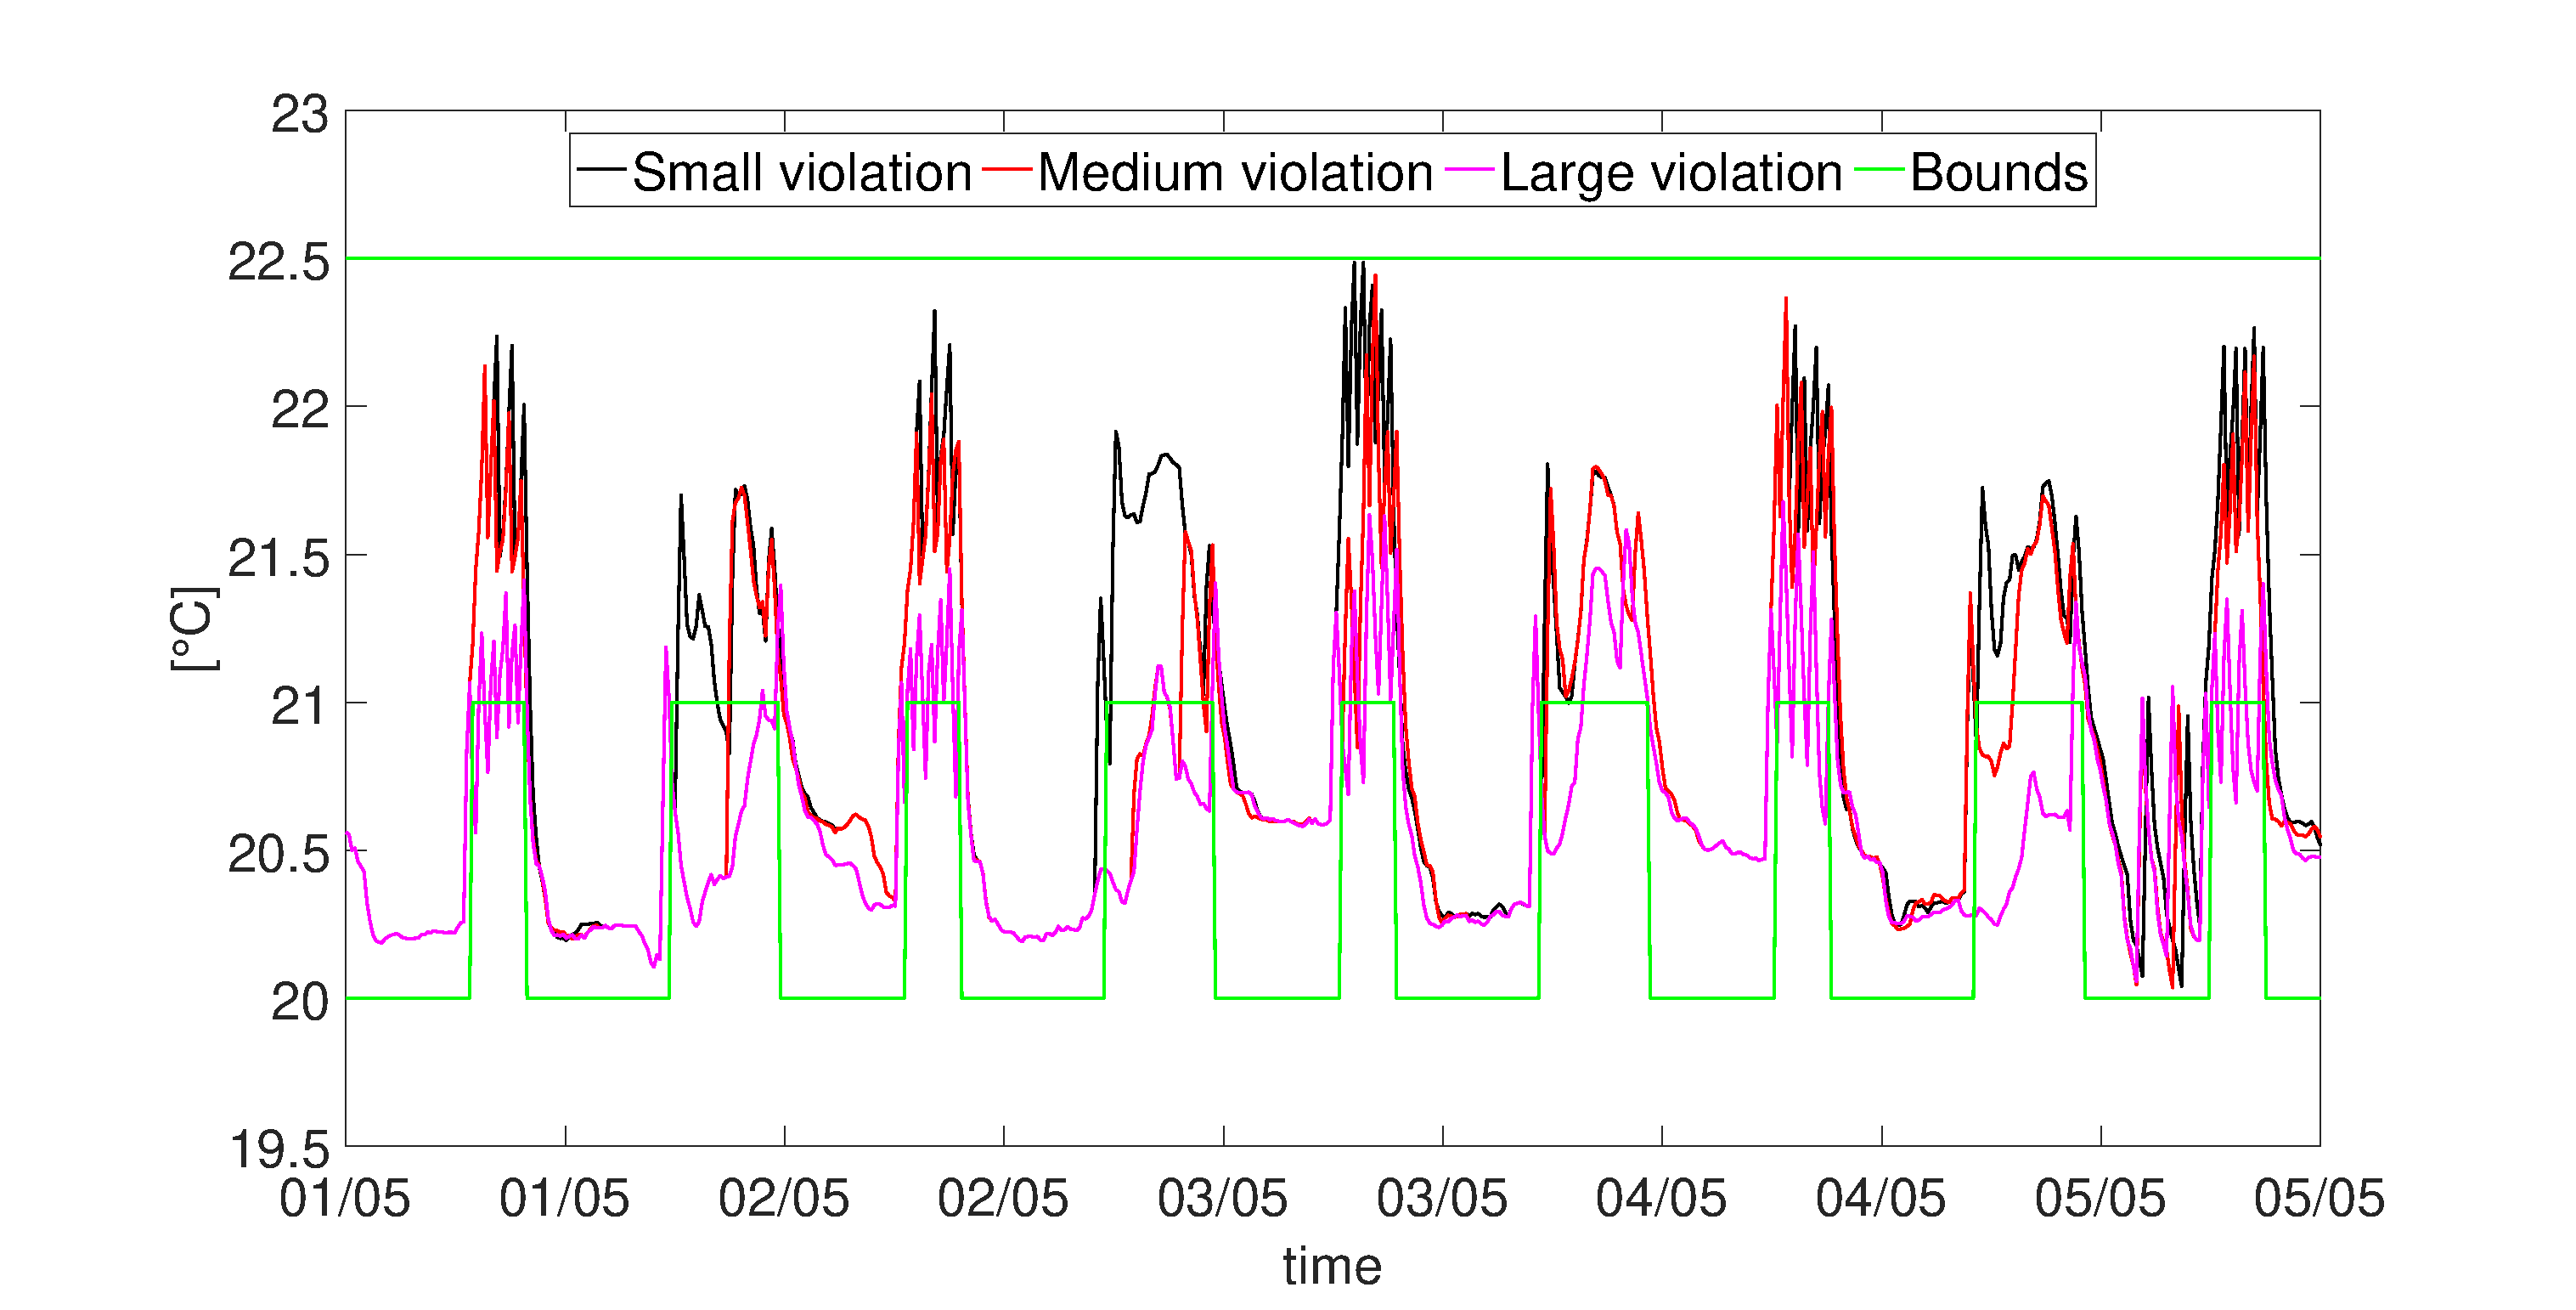
\includegraphics[width=22pc]{figures/Temperatures_all.eps}
	}
	\subfigure[Input schedules obtained from DPC and ON/OFF controller.]{
		\label{F:Energy_all}
		\centering
		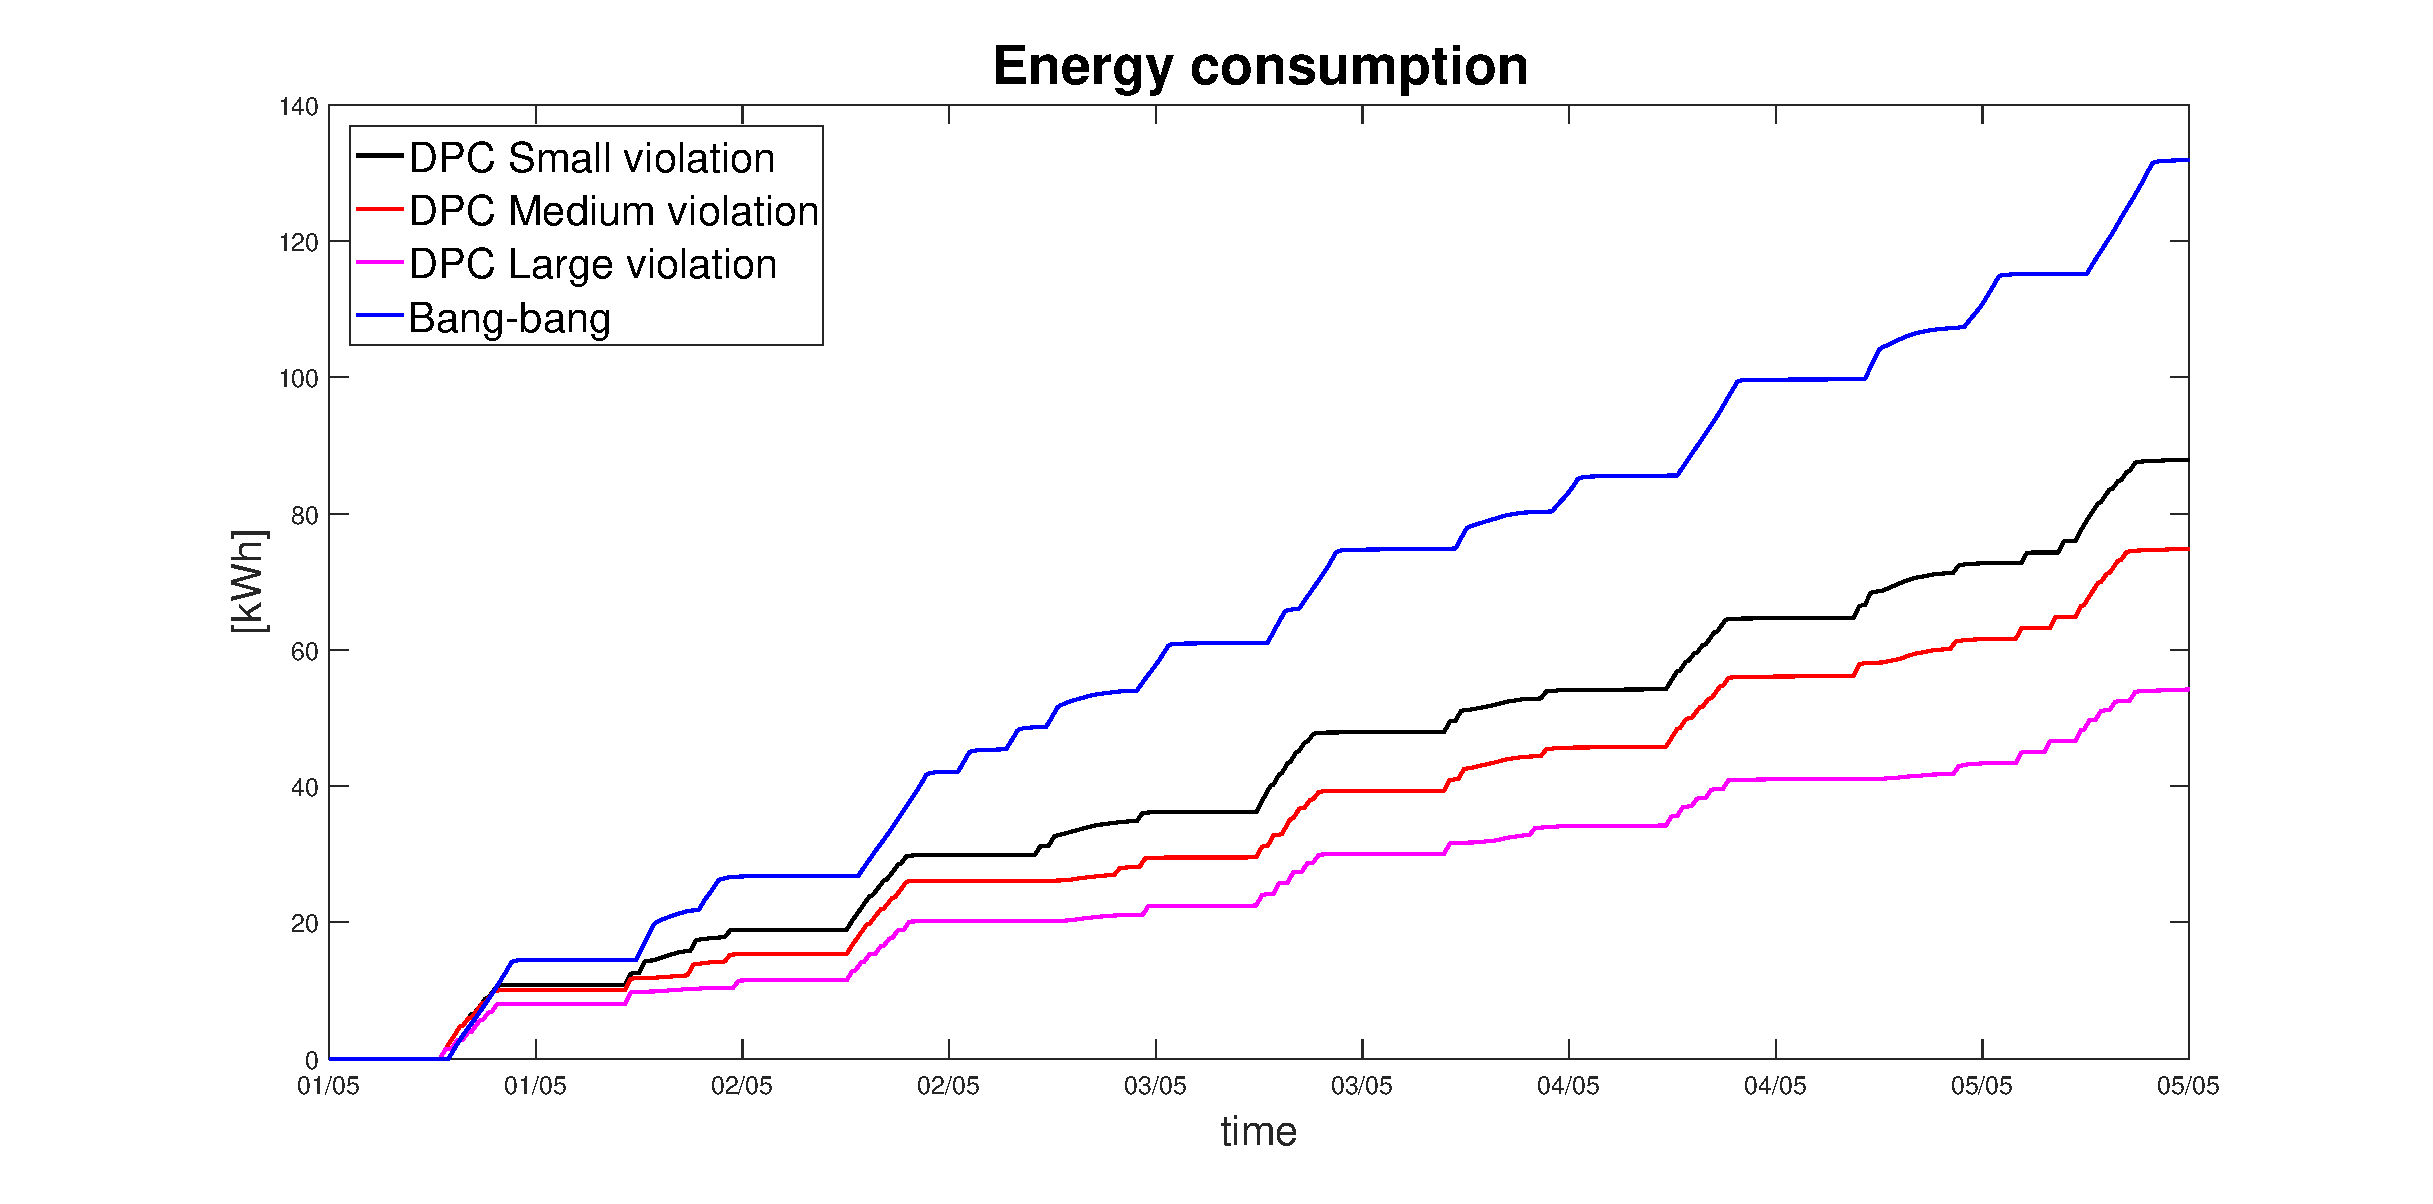
\includegraphics[width=22pc]{figures/Energy_all.eps}
	}
	\caption{Comparison of DPC and ON/OFF control performance with different violations.}
	\captionsetup{justification=centering}
	\label{F:Comparison_small}
\end{figure}
\paragraph{Energy-efficiency improvements}